% !TeX encoding = UTF-8

\documentclass{protokol}

\usepackage{tikz}
\usetikzlibrary{calc}
\usetikzlibrary{arrows}

%====== Units =====
\usepackage{siunitx}
\sisetup{inter-unit-product =\ensuremath{\cdot}}
\sisetup{group-digits = integer}
\sisetup{output-decimal-marker = {,}}
\sisetup{exponent-product = \ensuremath{\cdot}}
\sisetup{separate-uncertainty}
\sisetup{tight-spacing = false}
%\sisetup{scientific-notation = true}
%\sisetup{round-mode=places,round-precision=4}
%\sisetup{evaluate-expression}


%====== Grafy =====
\usepackage{pgfplots}
\pgfplotsset{width=0.8\linewidth, compat=1.17}
\def\plotcscale{0.8}
\usepackage{pgfplotstable}
\usepackage[figurename=Obr.]{caption} % figure caption rename
%====== Rovnice align block ======
\usepackage{amsmath}
\setlength{\jot}{10pt} % rozestup mezi řádky

\graphicspath{ {./img/} }

%====== Vyplňte údaje ======
\jmeno{Jakub Charvot}
\kod{240844}
\rocnik{2.}
\obor{MET}
\skupina{MET/4}
\spolupracoval{Radek Kučera}

\merenodne{10.\,11.\,2022}
\odevzdanodne{24.\,11.\,2022}
\nazev{Operační usměrňovače}
\cislo{4} %měřené úlohy

\predmet{Analogové elektronické obvody}
\ustav{Ústav mikroelektroniky}
\skola{FEKT VUT v Brně}

\def\para{x+0}
\def\parb{\para-80}

% CSV
\usepackage{blindtext}

\usepackage{subfiles} % Best loaded last in the preamble
\usepackage{datatool}


\DTLloaddb[omitlines=0]{namerene_hodnoty}{data/graf-na-U.csv}
\DTLloaddb{vykon}{data/vykon.csv}
\DTLloaddb{frekvence}{data/frekvence.csv}


\begin{document}
	%====== Vygenerování tabulky ======
%	\maketitle
	%====== Úvodní texty protokolu ======

%	\section{Teoretický úvod}
%		\begin{figure}[h!]
    \centering
    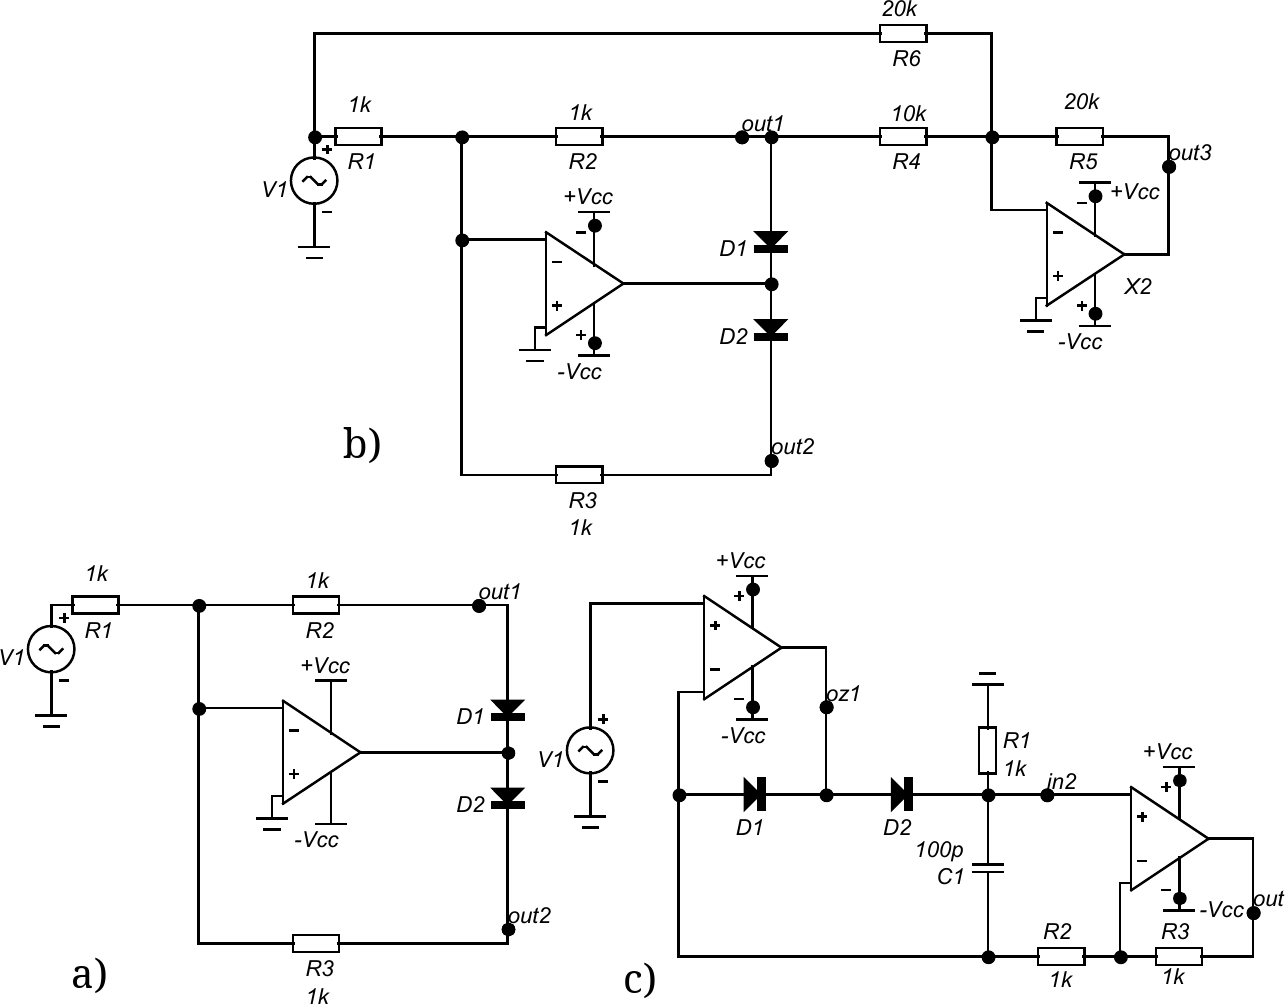
\includegraphics[width=\textwidth]{schema.png}
    \centering
    \caption{Schémata zapojení -- a) jednocestný usměrňovač, b) dvoucestný usměrňovač, c) dvoucestný usměrňovač s minimem přesných součástek.}
    \label{fig:schema}
\end{figure}



\subsection{Funkce jednotlivých zapojení}

    Operační zesilovač s OZ má za úkol překonat nedostatky, které má zapojení pouze s diodami, které díky svému prahovému napětí nedokáží usměrňovat velmi malá napětí. 
    
    Zapojení 1a) je jednocestný usměrňovač, kdy je vždy přes jednu diodu uzavřená záporná zpětná vazba a druhá dioda je uzavřená. Na výstupu je pak signál jednocestně usměrněný a invertovaný. 
    
    Zapojení 1b) pak tento signál zdvojnásobí a sečte s původním vstupním signálem, ve výsledku tedy původní záporné půlvlny zůstanou a kladné po sečtení odpovídají opět záporným. Výsledkem je tedy dvoucestně usměrněný invertovaný signál. 
    Nevýhodou tohoto zapojení je nutnost použít dva co nejshodnější odpory a k nim jeden, který odpovídá hodnotu přesně polovině, při nedodržení nebudou na výstupu půlvlny stejně velké, toto značně zdražuje zapojení. 

    Tento problém se snaží řešit zapojení 1c), kdy pro správnou funkci stačí jedna dvojice přesných odporů \( R_2\) a \(R_3\). Záporná zpětná vazba prvního OZ je vždy uzavřena přes druhý OZ, díky diodám je ale cesta zpětné vazby jiná pro kladný a pro záporný signál, takže ve výsledku je na výstupu druhého OZ signál vždy kladný, neboli dvoucestně usměrněný.   
%		
%	% \newpage
%	\section{Výsledky počítačové simulace}
%		\begin{figure}[h!]
    \centering
    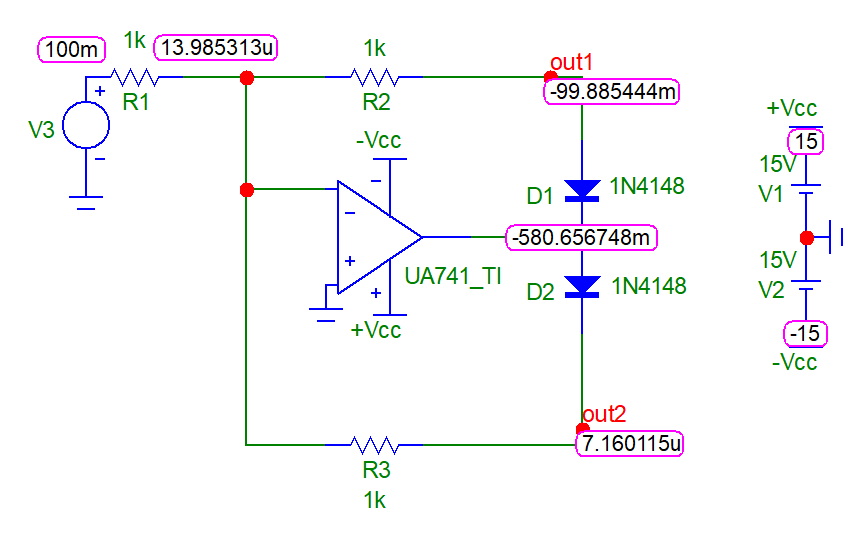
\includegraphics[width=0.63\textwidth]{microcap/1-dcbod.png}
    \caption{Zapojení a) -- stejnosměrný prac. bod pro kladné vstupní napětí.}
    \label{fig:microcap/.png}
\end{figure}

\begin{figure}[h!]
    \centering
    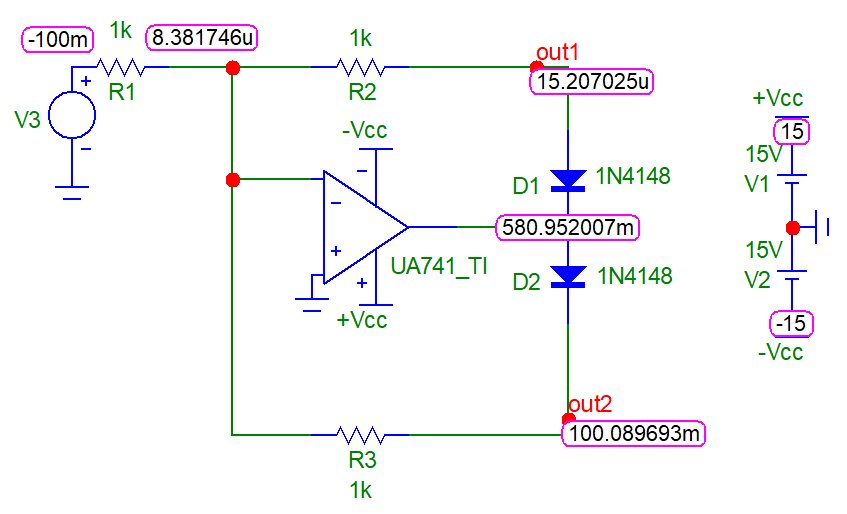
\includegraphics[width=0.63\textwidth]{microcap/1-dcbod2.png}
    \caption{Zapojení a) -- stejnosměrný prac. bod pro záporné vstupní napětí.}
    \label{fig:microcap/.png}
\end{figure}

\begin{figure}[h!]
    \centering
    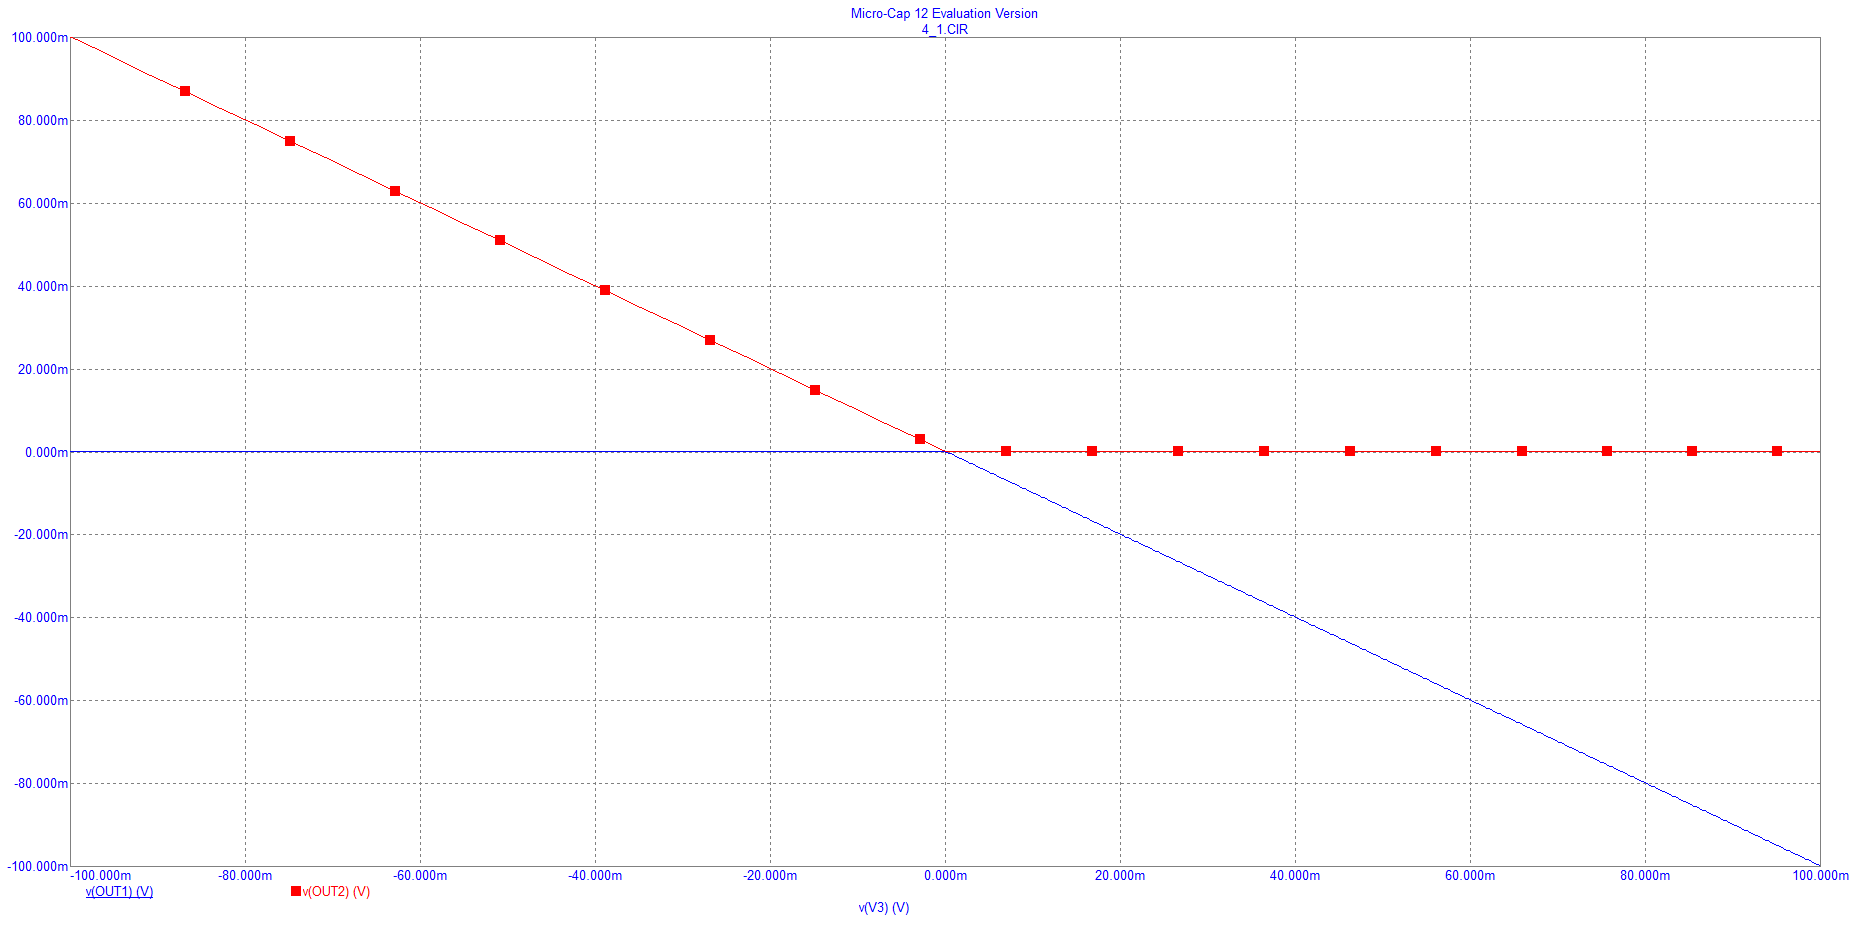
\includegraphics[width=0.8\textwidth]{microcap/1-dcprevodni.png}
    \caption{Zapojení a) -- stejnosměrná převodní charakteristika.}
    \label{fig:microcap/.png}
\end{figure}

\begin{figure}[h!]
    \centering
    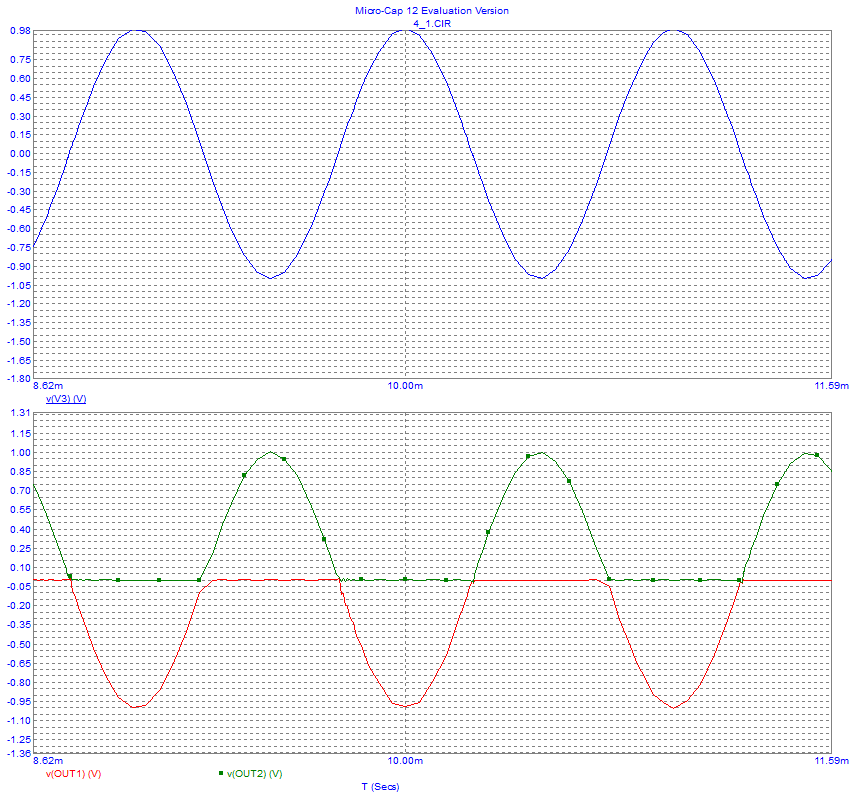
\includegraphics[width=0.8\textwidth]{microcap/1-transient-1khz-1v.png}
    \caption{Zapojení a) -- časová závislost obou výstupních napětí na vstupním napětí, jednocestné zesílení, \(f=\qty{1}{\kilo\hertz}, U_M=\qty{1}{\volt}\).}
    \label{fig:microcap/.png}
\end{figure}

\begin{figure}[h!]
    \centering
    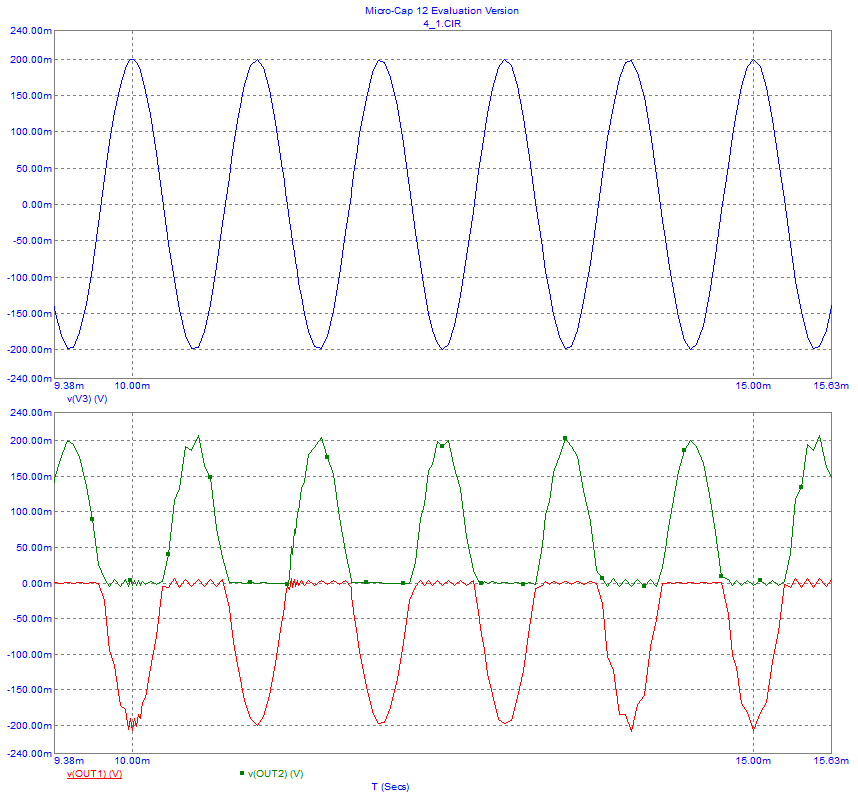
\includegraphics[width=0.7\textwidth]{microcap/1-transient-1khz-0.2v.png}
    \caption{Zapojení a) -- časová závislost obou výstupních napětí na vstupním napětí, nejmenší amplituda, při které zapojení obstojně usměrňuje, \(f=\qty{1}{\kilo\hertz}, U_M=\qty{200}{\milli\volt}\).}
    \label{fig:microcap/.png}
\end{figure}

\begin{figure}[h!]
    \centering
    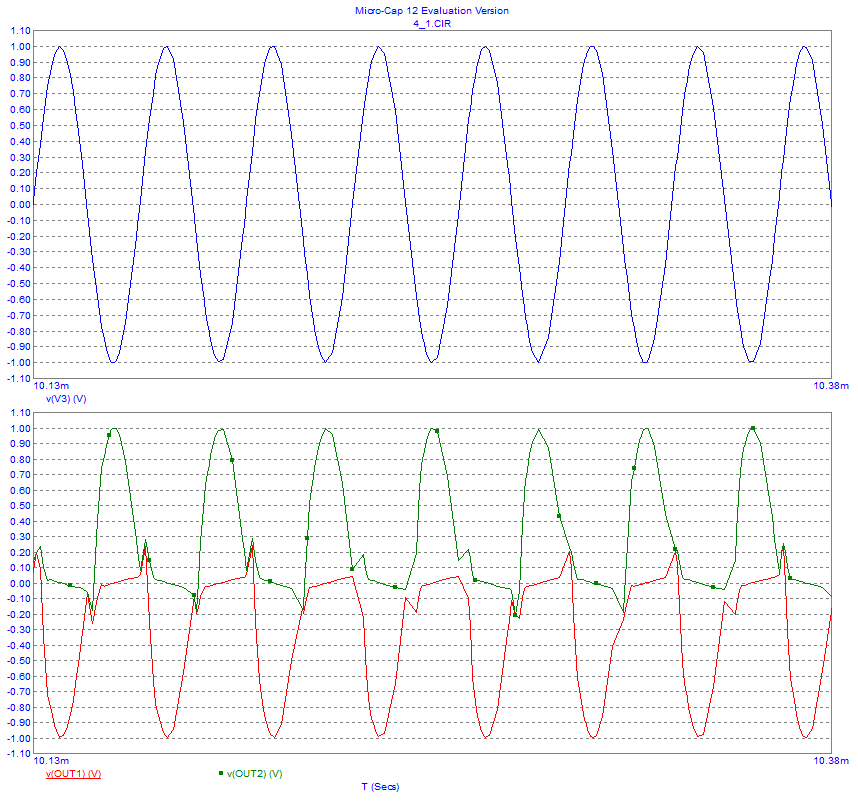
\includegraphics[width=0.7\textwidth]{microcap/1-transient-30khz-1v.png}
    \caption{Zapojení a) -- časová závislost obou výstupních napětí na vstupním napětí, nejvyšší frekvence, při které zapojení obstojně usměrňuje, \(f=\qty{30}{\kilo\hertz}, U_M=\qty{1}{\volt}\).}
    \label{fig:microcap/.png}
\end{figure}

\begin{figure}[h!]
    \centering
    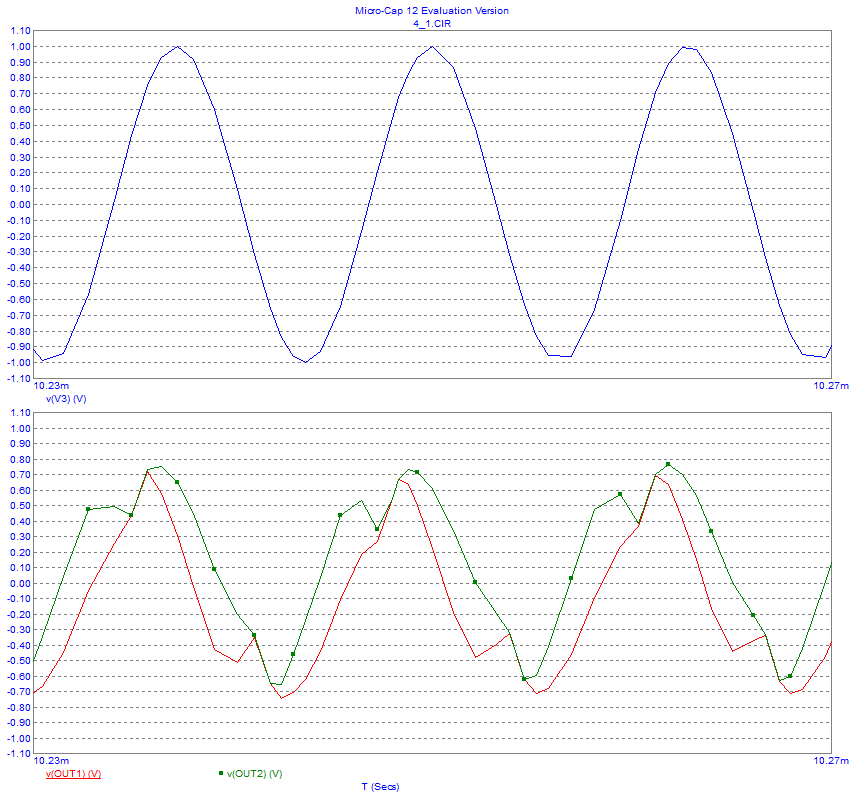
\includegraphics[width=0.8\textwidth]{microcap/1-transient-100khz-1v.png}
    \caption{Zapojení a) -- časová závislost obou výstupních napětí na vstupním napětí, příliš vysoká frekvence, k usměrnění nedochází vůbec, \(f=\qty{100}{\kilo\hertz}, U_M=\qty{1}{\volt}\).}
    \label{fig:microcap/.png}
\end{figure}    

% \begin{figure}[h!]
%     \centering
%     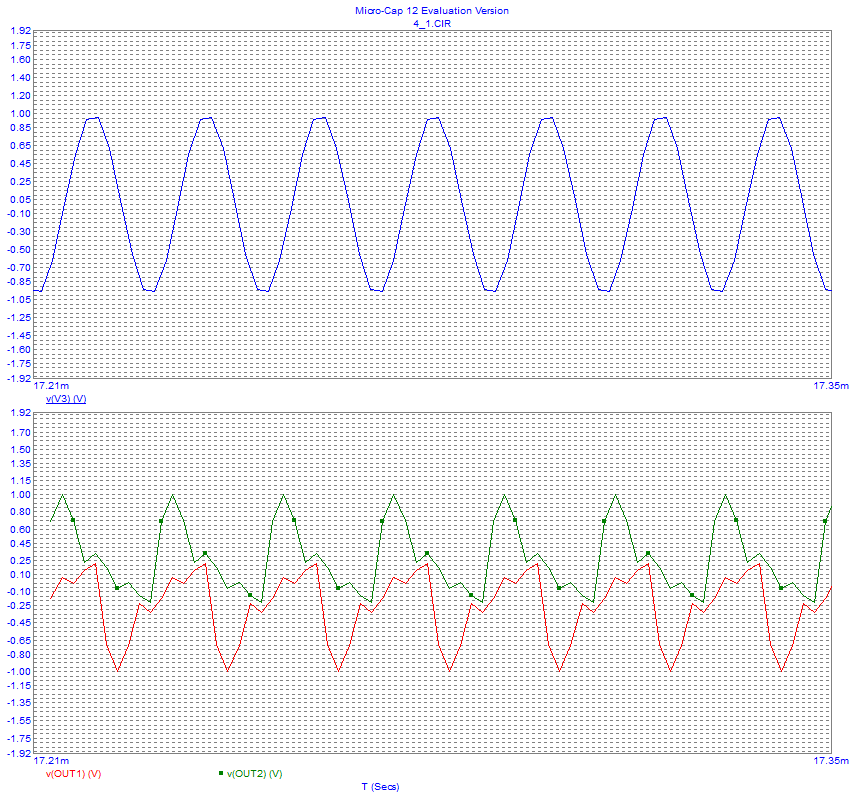
\includegraphics[width=0.8\textwidth]{microcap/1-transient-50khz-1v.png}
%     \caption{microcap/.png}
%     \label{fig:microcap/.png}
% \end{figure}

\begin{figure}[h!]
    \centering
    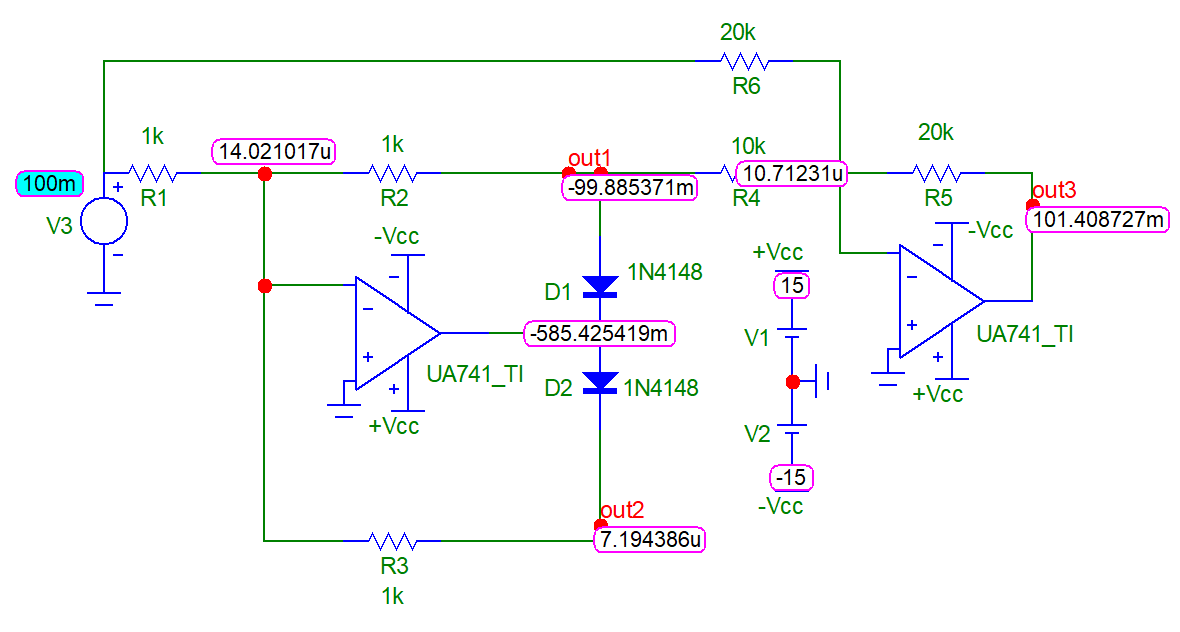
\includegraphics[width=0.8\textwidth]{microcap/2-dcbod.png}
    \caption{Zapojení b) -- stejnosměrný prac. bod při kladném napětí na vstupu, na výstupu kladné napětí.}
    \label{fig:microcap/.png}
\end{figure}

\begin{figure}[h!]
    \centering
    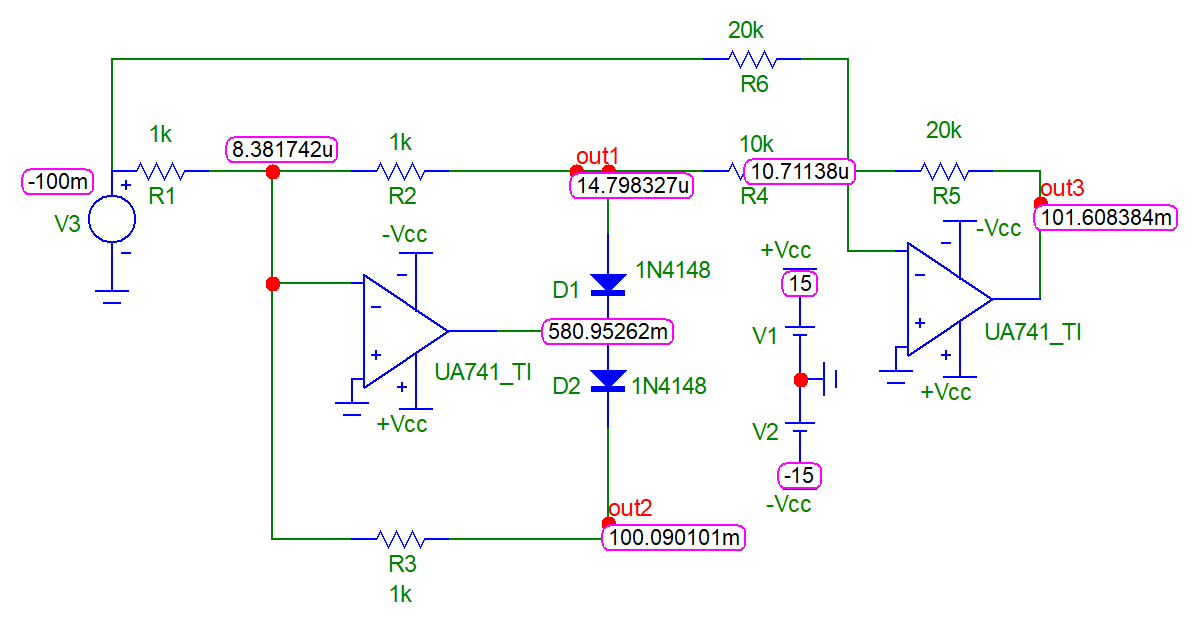
\includegraphics[width=0.61\textwidth]{microcap/2-dcbod2.png}
    \caption{Zapojení b) -- stejnosměrný prac. bod při záporném napětí na vstupu, na výstupu opět kladné napětí.}
    \label{fig:microcap/.png}
\end{figure}

\begin{figure}[h!]
    \centering
    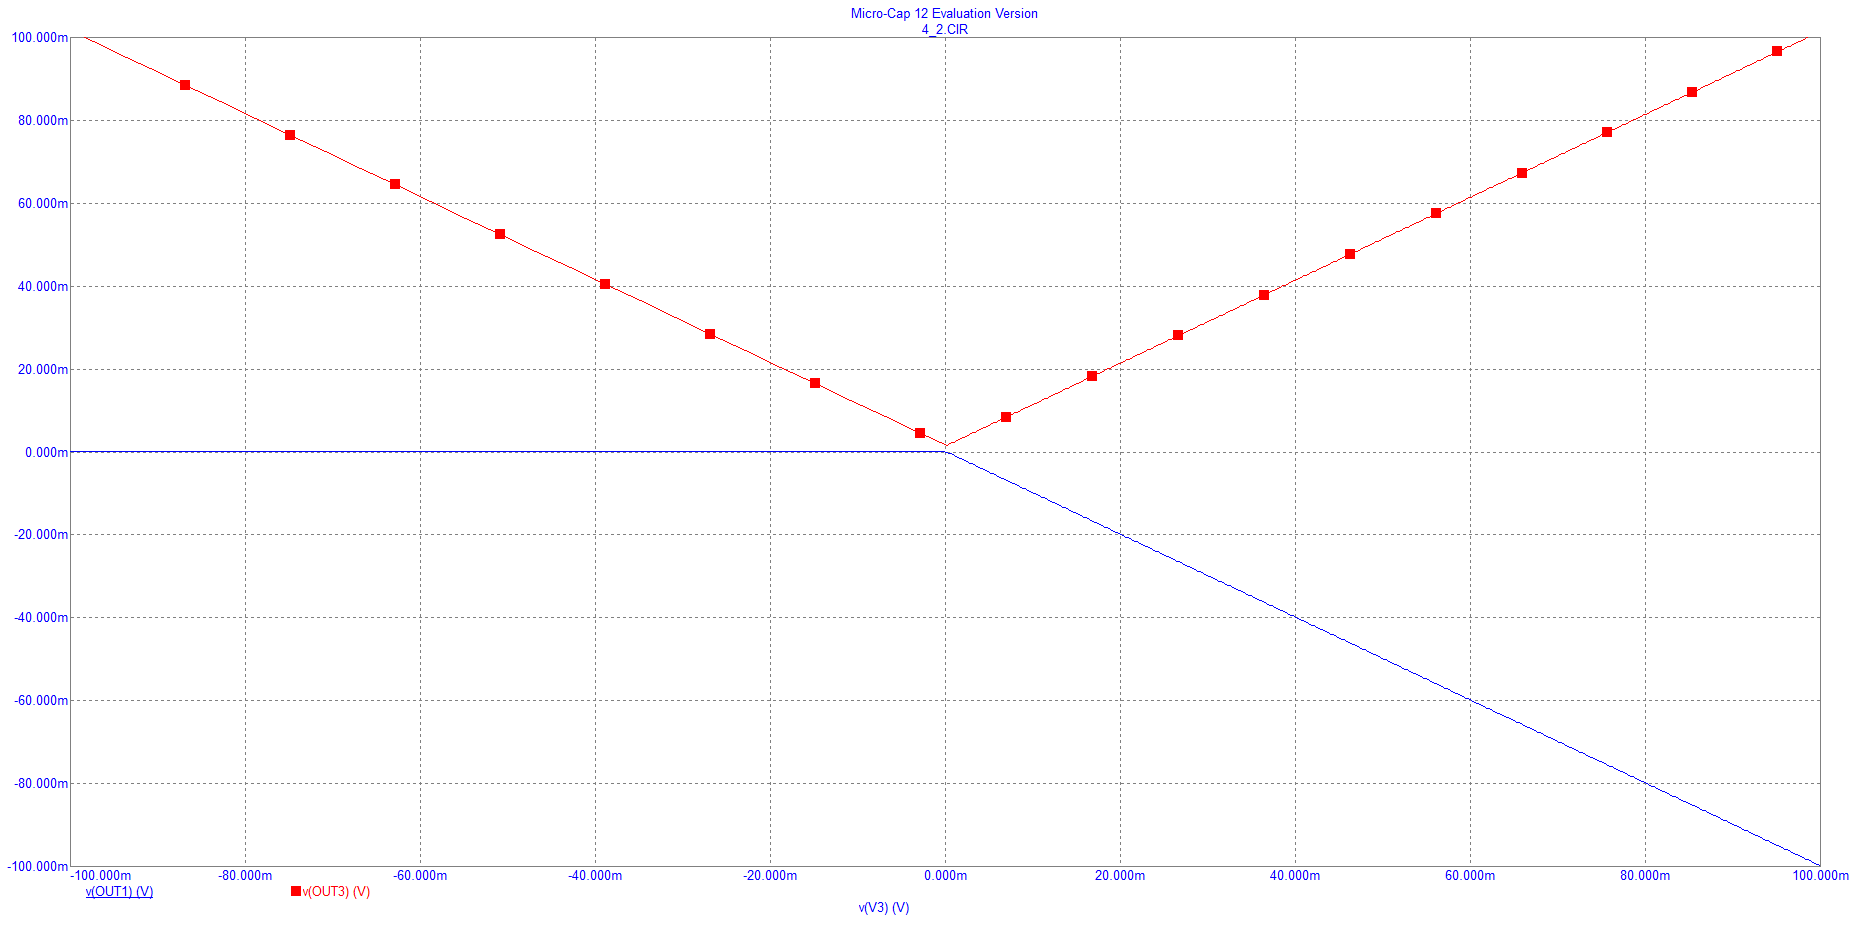
\includegraphics[width=0.61\textwidth]{microcap/2-dcprevodni.png}
    \caption{Zapojení b) -- stejnosměrná převodní charakteristika dvoucestného usměrnění.}
    \label{fig:microcap/.png}
\end{figure}

\begin{figure}[h!]
    \centering
    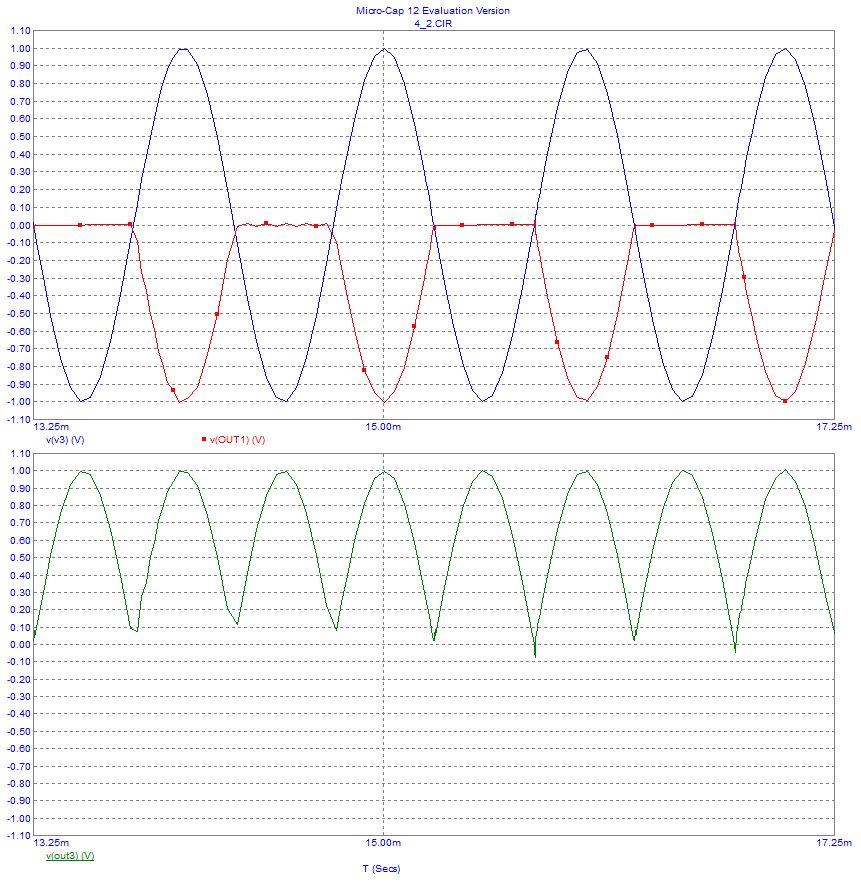
\includegraphics[width=0.61\textwidth]{microcap/2-transient-1khz-1v.png}
    \caption{Zapojení b) -- časová závislost napětí na výstupech obou OZ na vstupním napětí, jednocestné a dvoucestné usměrnění, \(f=\qty{1}{\kilo\hertz}, U_M=\qty{1}{\volt}\).}
    \label{fig:microcap/.png}
\end{figure}

% \begin{figure}[h!]
%     \centering
%     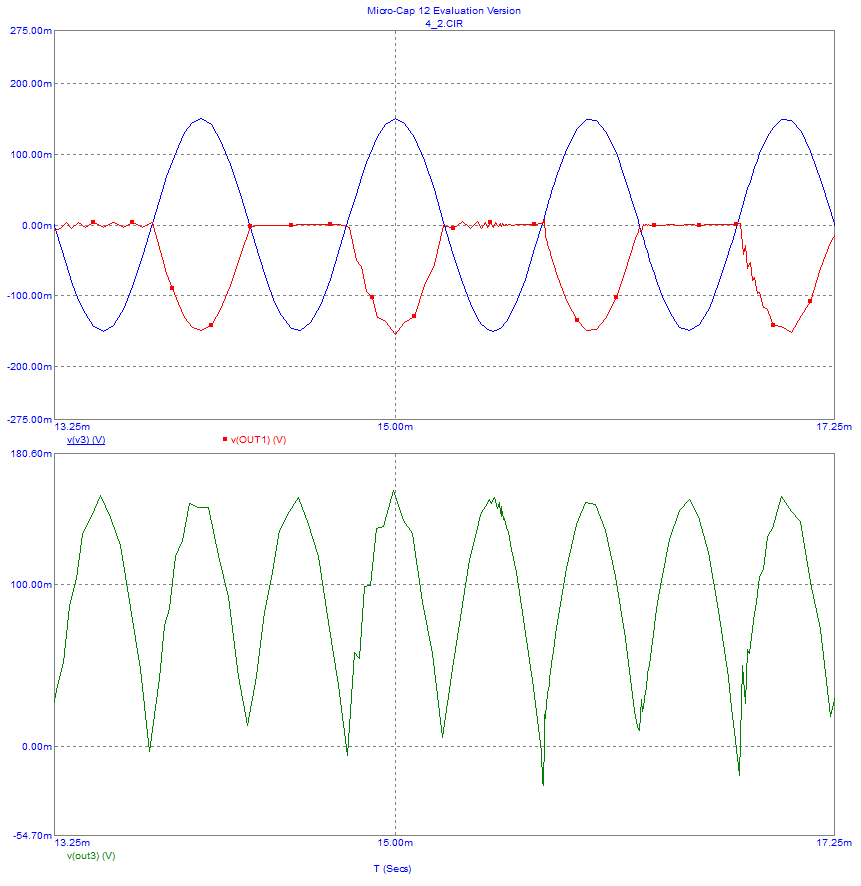
\includegraphics[width=0.8\textwidth]{microcap/2-transient-1khz-0.15v.png}
%     \caption{Zapojení b) -- časová závislost napětí na výstupech obou OZ na vstupním napětí, nejmenší amplituda, při které uspokojivě usměrňuje, \(f=\qty{1}{\kilo\hertz}, U_M=\qty{150}{\milli\volt}\).}
%     \label{fig:microcap/.png}
% \end{figure}

\begin{figure}[h!]
    \centering
    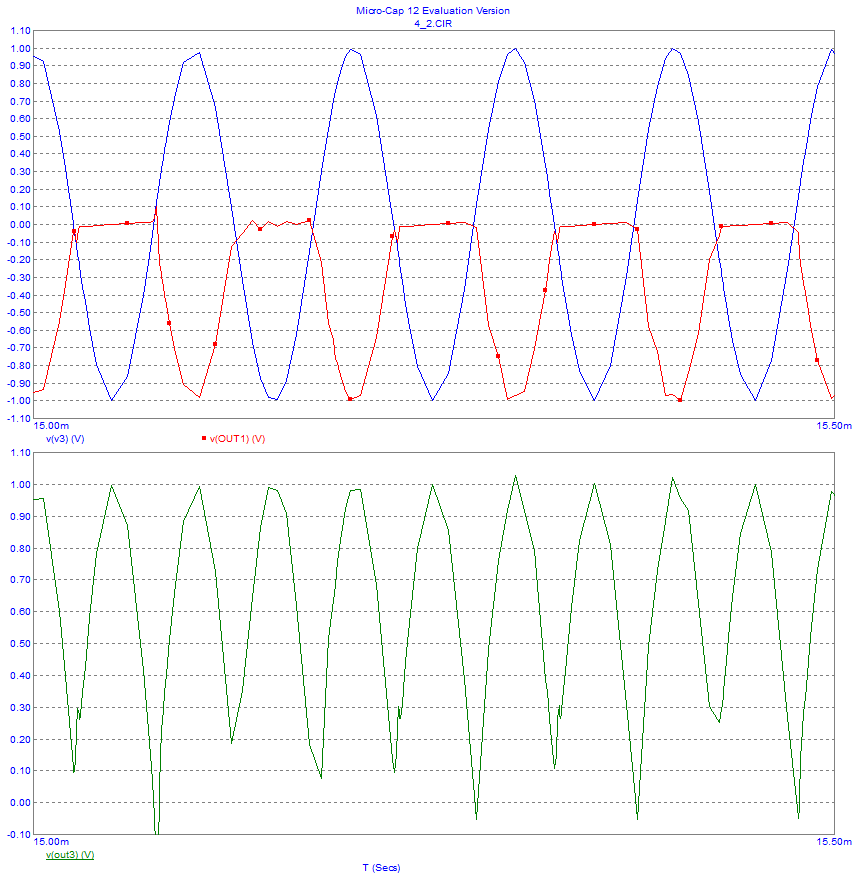
\includegraphics[width=0.7\textwidth]{microcap/2-transient-10khz-1v.png}
    \caption{Zapojení b) -- časová závislost napětí na výstupech obou OZ na vstupním napětí, nejvyšší frekvence, při které uspokojivě usměrňuje, \(f=\qty{10}{\kilo\hertz}, U_M=\qty{1}{\volt}\).}
    \label{fig:microcap/.png}
\end{figure}

\begin{figure}[h!]
    \centering
    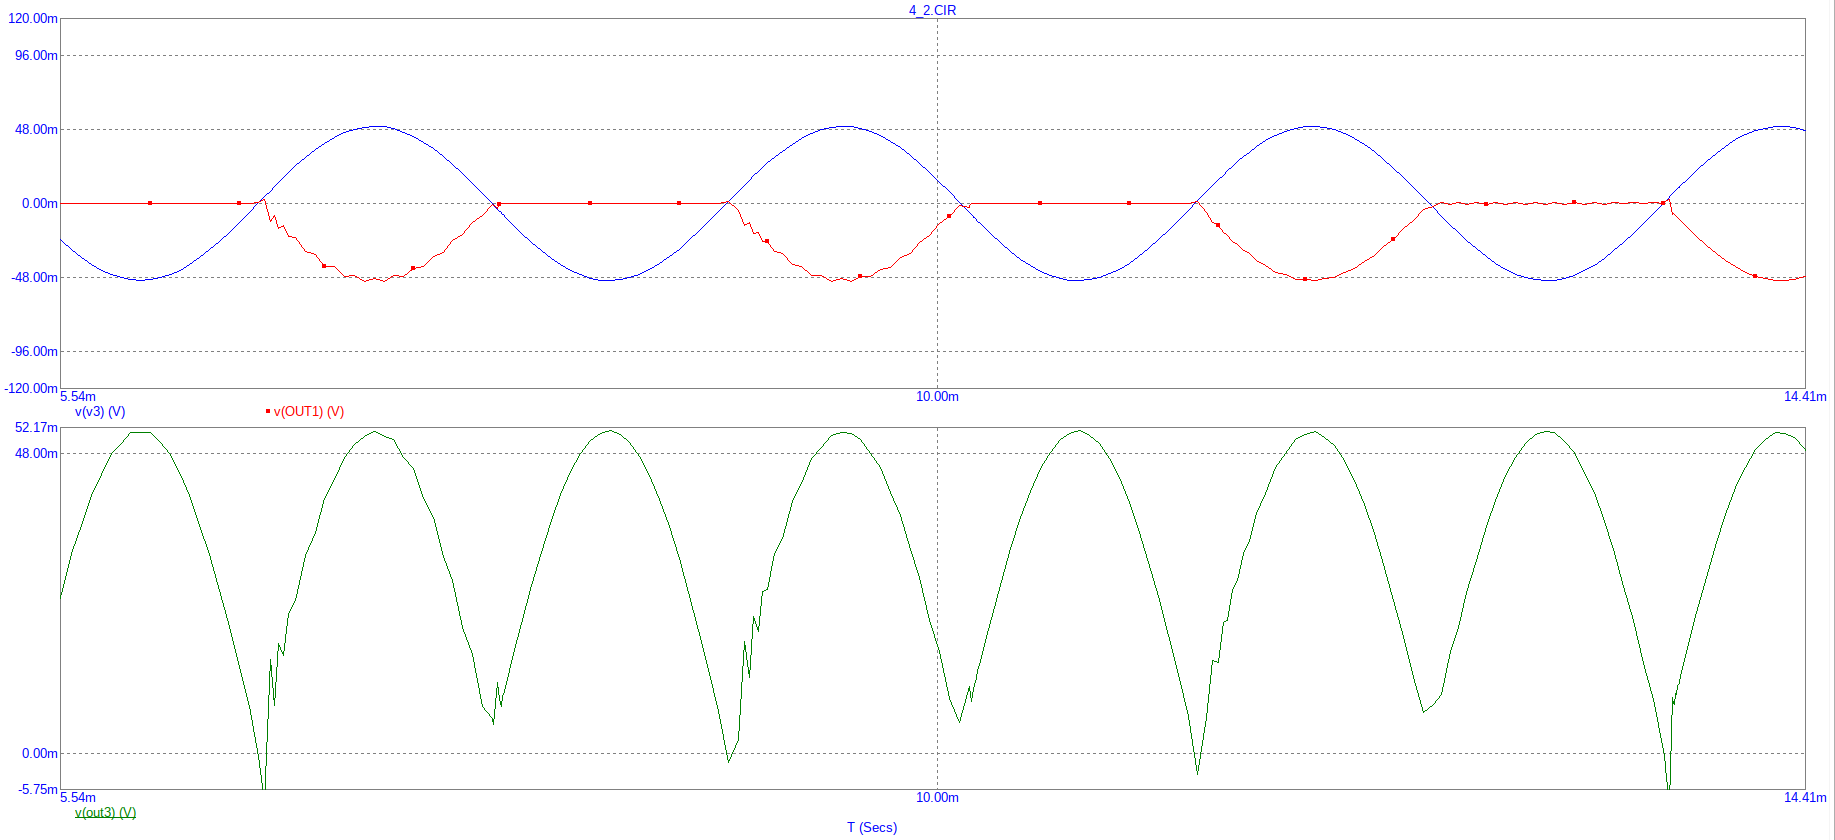
\includegraphics[width=0.7\textwidth]{microcap/2-transient-420hz-0.05v.png}
    \caption{Zapojení b) -- časová závislost napětí na výstupech obou OZ na vstupním napětí, nejnižší amplituda, při které uspokojivě usměrňuje, \(f=\qty{420}{\hertz}, U_M=\qty{50}{\milli\volt}\).}
    \label{fig:microcap/.png}
\end{figure}

\begin{figure}[h!]
    \centering
    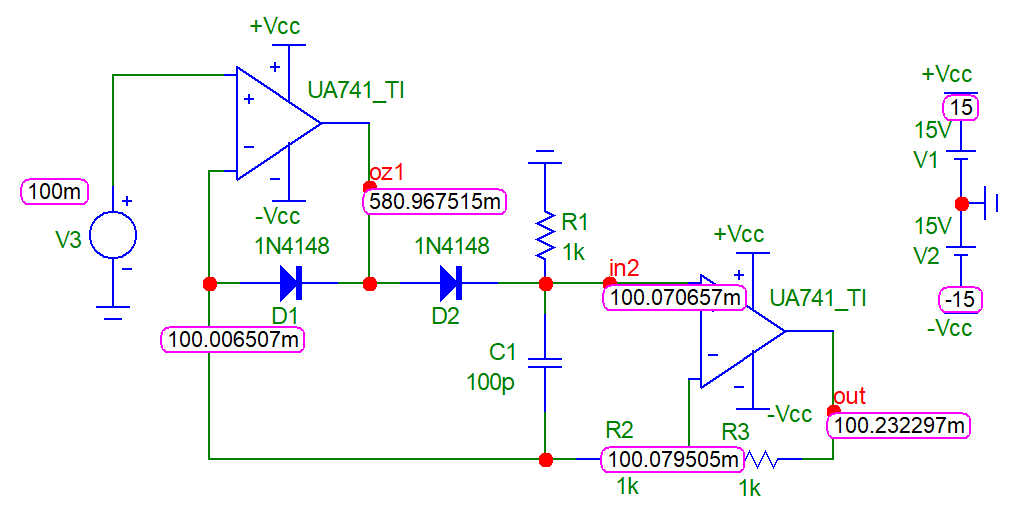
\includegraphics[width=0.8\textwidth]{microcap/3-dcbod.png}
    \caption{Zapojení c) -- stejnosměrný prac. bod při kladném napětí na vstupu, na výstupu kladné napětí.}
    \label{fig:microcap/.png}
\end{figure}

\begin{figure}[h!]
    \centering
    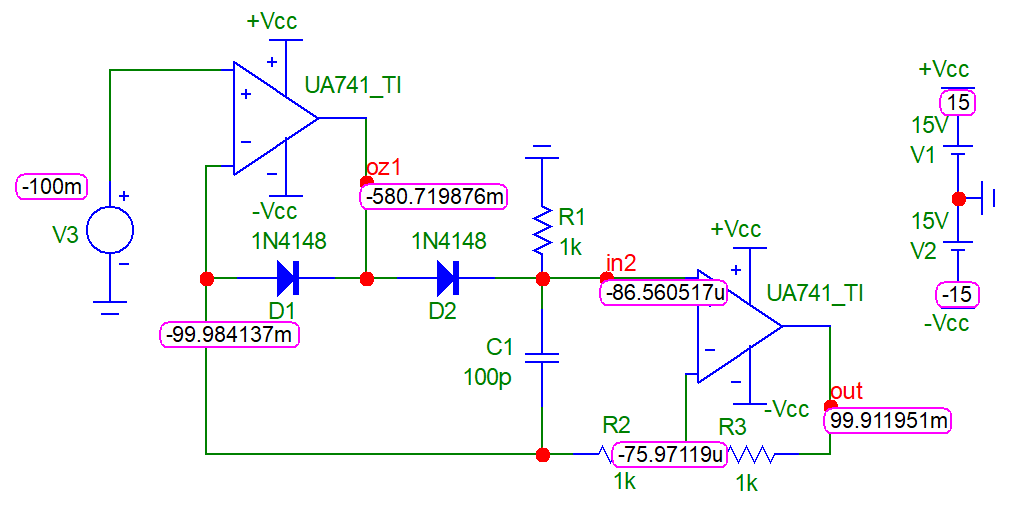
\includegraphics[width=0.8\textwidth]{microcap/3-dcbod2.png}
    \caption{Zapojení c) -- stejnosměrný prac. bod při záporném napětí na vstupu, na výstupu kladné napětí.}
    \label{fig:microcap/.png}
\end{figure}

\begin{figure}[h!]
    \centering
    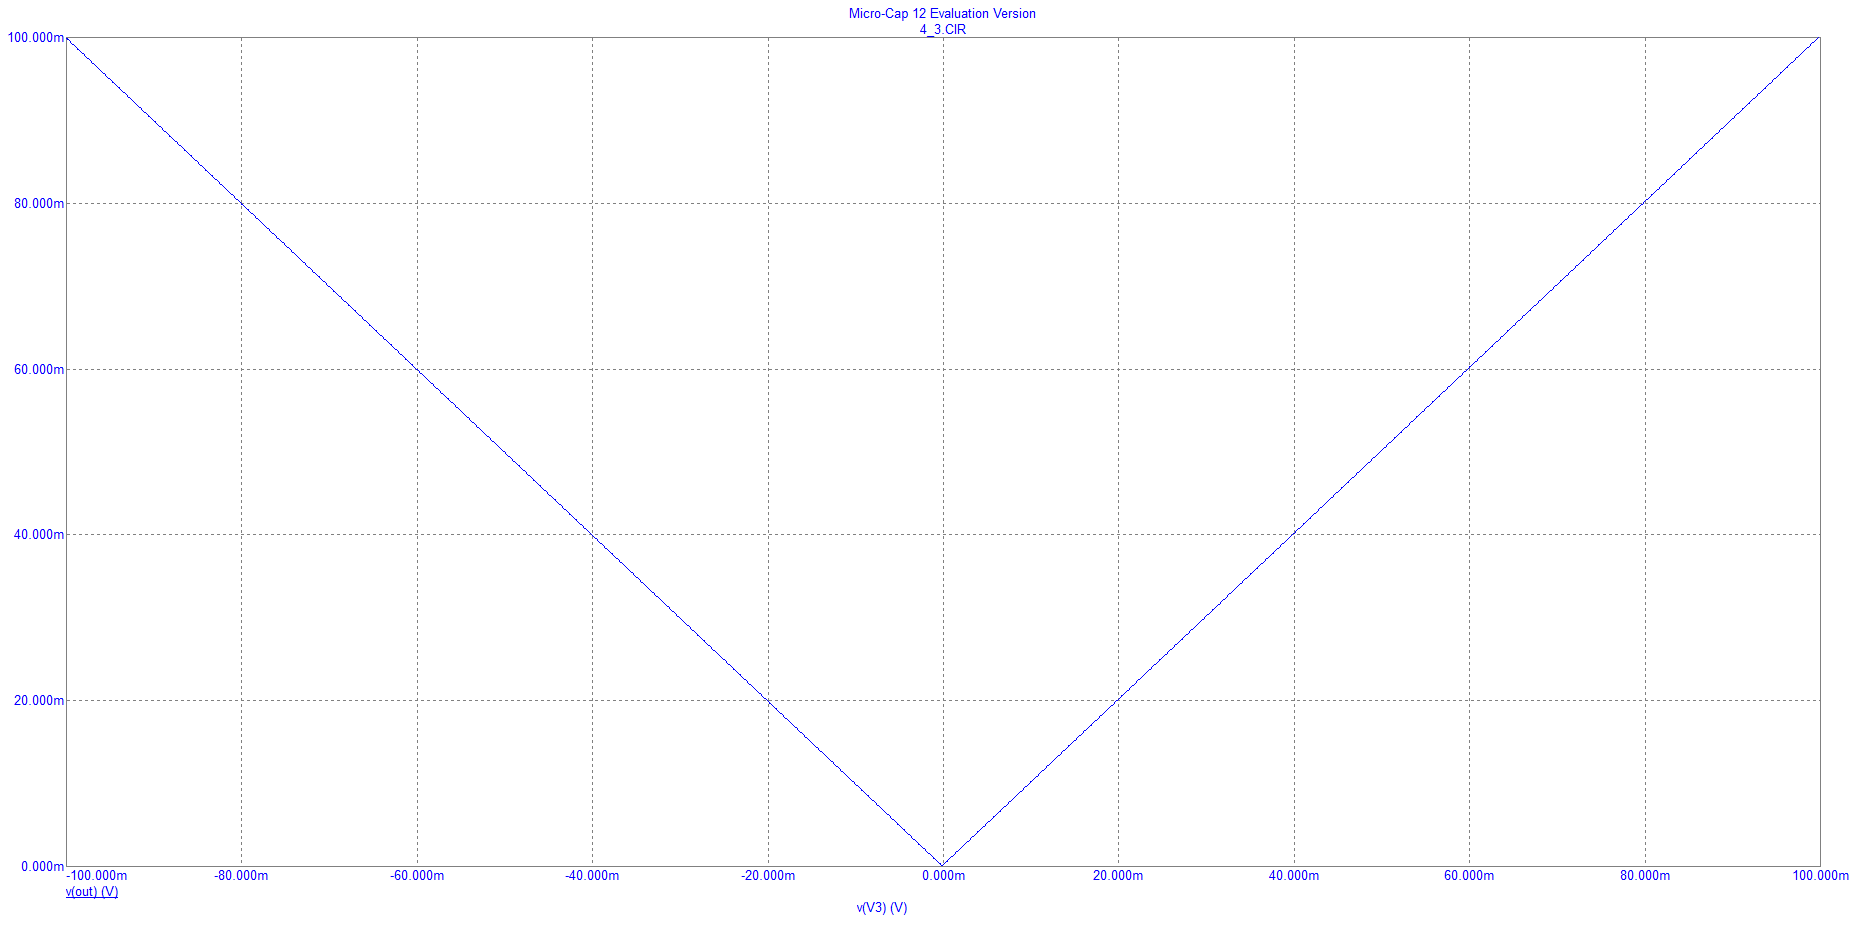
\includegraphics[width=0.8\textwidth]{microcap/3-dcprevodni.png}
    \caption{Zapojení c) -- stejnosměrná převodní charakteristika.}
    \label{fig:microcap/.png}
\end{figure}

\begin{figure}[h!]
    \centering
    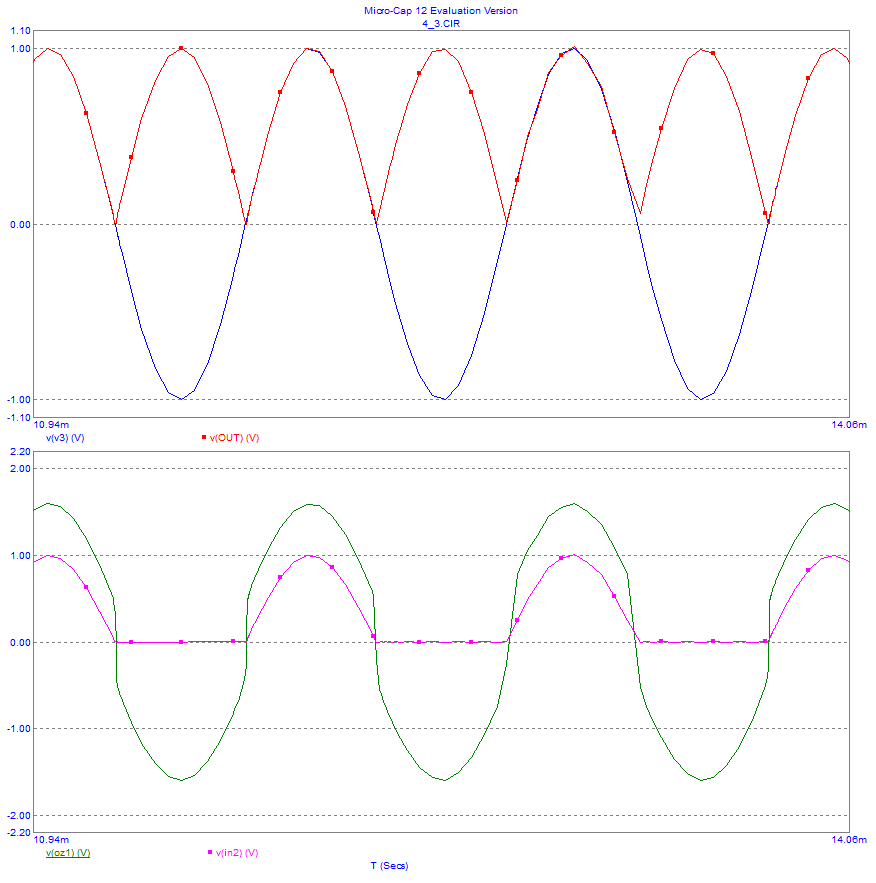
\includegraphics[width=0.66\textwidth]{microcap/3-transient-1khz-1v.png}
    \caption{Zapojení c) -- časová závislost napětí na výstupech obou OZ na vstupním napětí, jednocestné a dvoucestné usměrnění, \(f=\qty{1}{\kilo\hertz}, U_M=\qty{1}{\volt}\).}
    \label{fig:microcap/.png}
\end{figure}

\begin{figure}[h!]
    \centering
    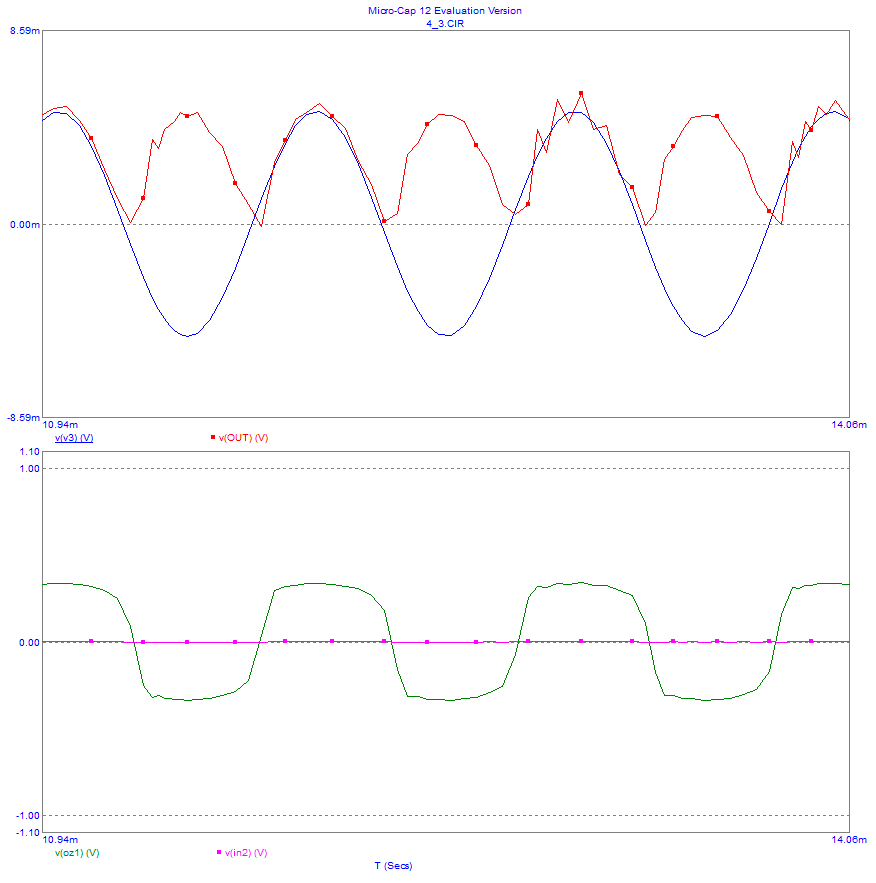
\includegraphics[width=0.66\textwidth]{microcap/3-transient-1khz-5mv.png}
    \caption{Zapojení c) -- časová závislost napětí na výstupech obou OZ na vstupním napětí, nejnižší amplituda, při které uspokojivě usměrňuje, \(f=\qty{1}{\kilo\hertz}, U_M=\qty{5}{\milli\volt}\).}
    \label{fig:microcap/.png}
\end{figure}

% \begin{figure}[h!]
%     \centering
%     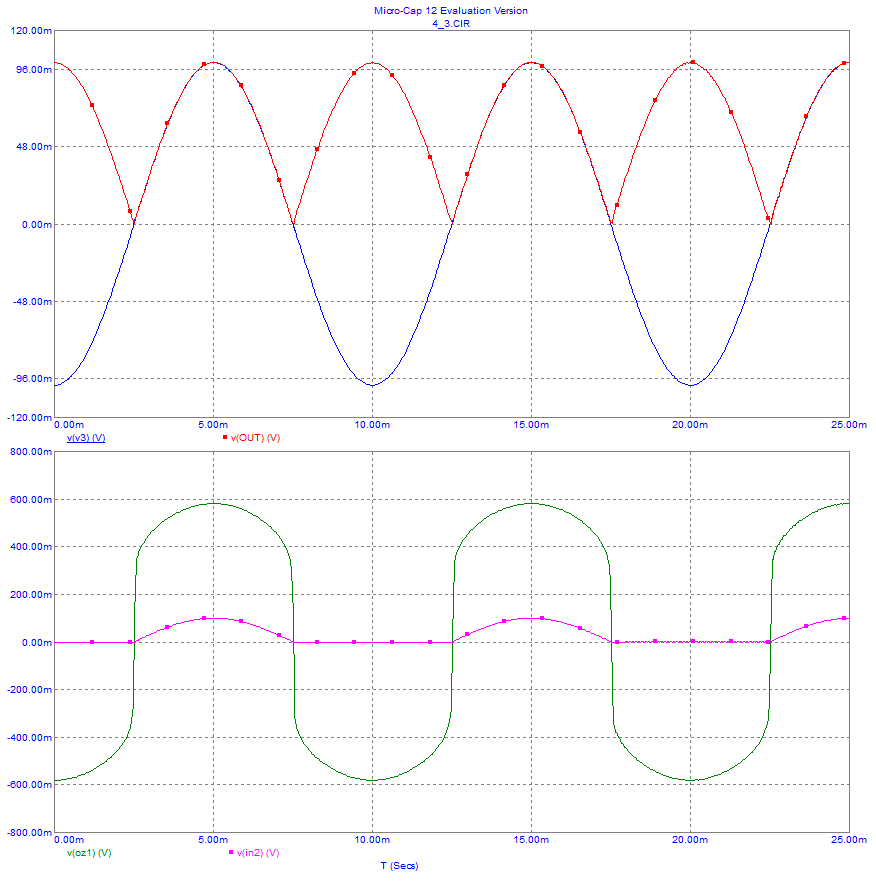
\includegraphics[width=0.8\textwidth]{microcap/3-transient-100hz-0.1v.png}
%     \caption{microcap/.png}
%     \label{fig:microcap/.png}
% \end{figure}

\begin{figure}[h!]
    \centering
    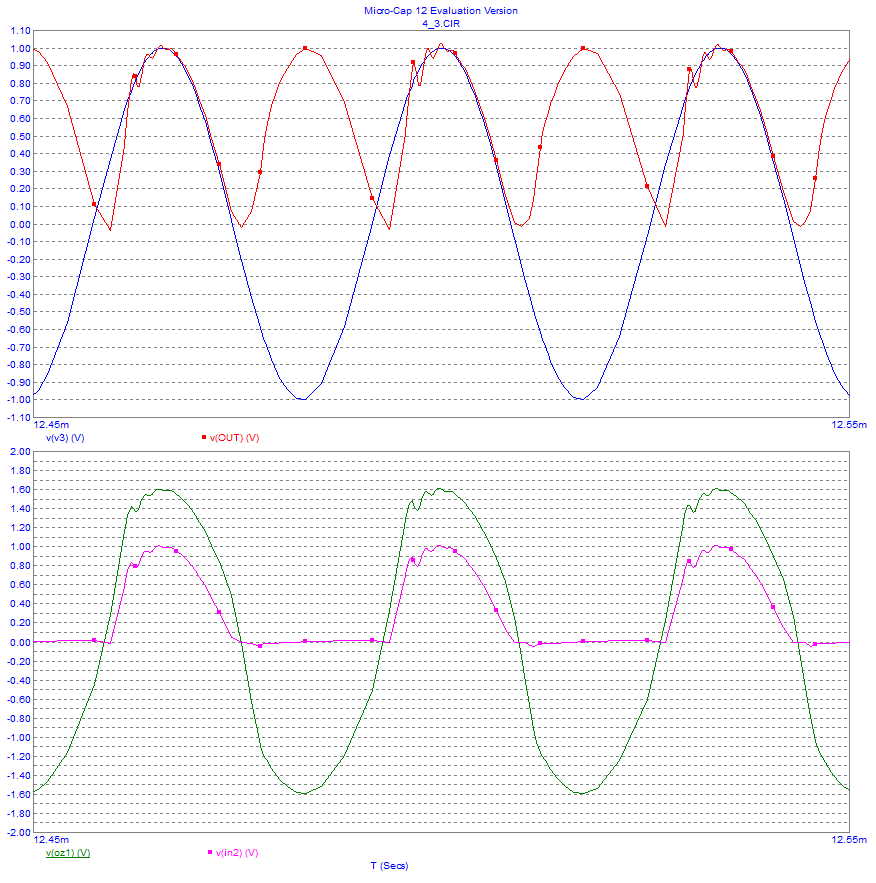
\includegraphics[width=0.8\textwidth]{microcap/3-transient-30khz-1v.png}
    \caption{Zapojení c) -- časová závislost napětí na výstupech obou OZ na vstupním napětí, nejvyšší frekvence, při které uspokojivě usměrňuje, \(f=\qty{30}{\kilo\hertz}, U_M=\qty{1}{\volt}\).}
    \label{fig:microcap/.png}
\end{figure}


%		
%	\clearpage
	\section{3.}
	V tabulce \ref{tab:tabulka-hodnot} se nachází hodnoty rychlosti větru naměřené anemometrem a otáčky vrtulky, které odpovídají polovině hodnoty naměřené otáčkoměrem.
	\begin{table}[h!]
		\centering
		\def\arraystretch{1.4}
		\begin{tabular}{ |l|l|l| }
			\hline
			U\ [\unit{\volt}] & $ v_{air} $\ [\unit{\meter\per\second}] & $ n_t $\ [\unit{\per\minute}]
			\DTLforeach{namerene_hodnoty}{\A=U,\B=v_air,\C=RPM}
			{\DTLiffirstrow{\\ \hline \hline}{\\ \hline} %
				\A & \num[round-mode=places,round-precision=2]{\B} & \num[round-mode=places,round-precision=1]{\C}}\\ \hline
		\end{tabular}
		\caption{\label{tab:tabulka-hodnot} Tabulka naměřených a vypočtených hodnot.}
	\end{table}

		\begin{figure*}[h!]
		\begin{tikzpicture}
			\centering
			\begin{axis}
				[
				xlabel={$U\ [\unit{\volt}]$},
				ylabel={$v_{air}[\unit{\meter\per\second}]$},
				width=1\textwidth,
				height = 0.5\textwidth,
				legend pos=south east,
				xmin=0,
				ymin=0,
				xmax=12.5
				]
				\addplot[mark=x, thick, blue, only marks, mark size=3pt] table [skip first n=0, x=U, y=v_air, col sep=comma] {data/graf-na-U.csv};
				
				%			\addlegendentry{Naměřené hodnoty}
				
			\end{axis}    
		\end{tikzpicture}
		\caption{Závislost rychlosti větru $ v_{air} $ na napětí zdroje.}
	\end{figure*}

	\begin{figure*}[h!]
		\begin{tikzpicture}
			\centering
			\begin{axis}
				[
				xlabel={$U\ [\unit{\volt}]$},
				ylabel={$n_t [\unit{\per\minute}]$},
				width=1\textwidth,
				height = 0.5\textwidth,
				legend pos=south east,
				xmin=0,
				ymin=0,
				xmax=12.5
				]
				\addplot[mark=x, thick, blue, only marks, mark size=3pt] table [skip first n=0, x=U, y=RPM, col sep=comma] {data/graf-na-U.csv};
				
				%			\addlegendentry{Naměřené hodnoty}
				
			\end{axis}    
		\end{tikzpicture}
		\caption{Závislost otáček $ n_t $ vrtulky na napětí zdroje.}
	\end{figure*}

\section{4.}
	\begin{table}[h!]
		\centering
		\def\arraystretch{1.4}
		\begin{tabular}{ |l|l|l|l|l| }
			\hline
			U\ [\unit{\volt}] & I\ [\unit{\ampere}] & $ P_{in} $\ [\unit{\watt}] & $ P_{V} $\ [\unit{\watt}] & $ \eta $\ [\unit{\percent}] 
			\DTLforeach{vykon}{\A=U,\B=I,\C=Pin,\D=Pv,\E=etha}
			{\DTLiffirstrow{\\ \hline \hline}{\\ \hline} %
				\A & \num[round-mode=places,round-precision=2]{\B} & \num[round-mode=places,round-precision=2]{\C} & \num{\D} & \num{\E}}\\ \hline
		\end{tabular}
		\caption{\label{tab:tabulka-vykon} Tabulka naměřených a vypočtených hodnot.}
	\end{table}

Příklady výpočtu:

$$ P_{in}=U\cdot I=6\cdot 0,33 \doteq \SI{1,98}{\watt}$$
$$ P_{V}=\frac{1}{2}\cdot \rho \cdot{v_{air}}^3 \cdot A = \frac{1,29\cdot 1,9^3 \cdot\pi\cdot 0,1^2}{2}\doteq \SI{0,139}{\watt}$$
$$ \eta = \frac{P_V}{P_{in}} \cdot 100=\frac{1,98}{0,139}\doteq \SI{7,02}{\percent}$$

\clearpage
\section{7. a 8.}
	\begin{table}[h!]
		\centering
		\def\arraystretch{1.4}
		\begin{tabular}{ |l|l|l|l|l| }
			\hline
			$ U_{in} $\ [\unit{\volt}] & f\ [\unit{\hertz}] & $ U_{OUT(p-p)} $\ [\unit{\volt}] & $ n_{g} $\ [\unit{\per\minute}] & $ p $\ [--] 
			\DTLforeach{frekvence}{\A=Uin,\B=f,\C=Uout,\D=RPM,\E=p}
			{\DTLiffirstrow{\\ \hline \hline}{\\ \hline} %
				\A & \num[round-mode=places,round-precision=2]{\B} & \num[round-mode=places,round-precision=2]{\C} & \num{\D} & \num{\E}}\\ \hline
		\end{tabular}
		\caption{\label{tab:tabulka-frekvence} Tabulka naměřených a vypočtených hodnot.}
	\end{table}

Výpočet počtu pólových dvojic:
$$ p=\frac{60f}{n_g}=\frac{60\cdot 4,5}{57}\doteq 4,74 $$
Průměrem vypočtených hodnot je číslo 5,66 $\approx$ 6, tolik pólových dvojic odhaduji v motoru.

	\begin{figure*}[h!]
	\begin{tikzpicture}
		\centering
		\begin{axis}
			[
			ylabel={$U_{OUT(p-p)}\ [\unit{\volt}]$},
			xlabel={$n_g [\unit{\per\minute}]$},
			width=1\textwidth,
			height = 0.5\textwidth,
			legend pos=south east,
			xmin=0,
			ymin=0,
%			xmax=12.5
			]
			\addplot[mark=x, thick, blue, only marks, mark size=3pt] table [skip first n=0, x=RPM, y=U_out, col sep=comma] {data/grafy2.csv};
			
			%			\addlegendentry{Naměřené hodnoty}
			
		\end{axis}    
	\end{tikzpicture}
	\caption{Závislost výstupního napětí generátoru $ U_{OUT(p-p)} $ na otáčkách vrtulky generátoru.}
\end{figure*}

\clearpage
\section{9.}
	\begin{figure*}[h!]
	\begin{tikzpicture}
		\centering
		\begin{axis}
			[
			ylabel={$U_{OUT(p-p)}\ [\unit{\volt}]$},
			xlabel={$v_{air} [\unit{\meter\per\second}]$},
			width=1\textwidth,
			height = 0.5\textwidth,
			legend pos=south east,
			xmin=0,
			ymin=0,
%			xmax=12.5
			]
			\addplot[mark=x, thick, blue, only marks, mark size=3pt] table [skip first n=0, x=v_air, y=U_out, col sep=comma] {data/grafy2.csv};
			
			%			\addlegendentry{Naměřené hodnoty}
			
		\end{axis}    
	\end{tikzpicture}
	\caption{Závislost výstupního napětí generátoru $ U_{OUT(p-p)} $ na rychlosti větru.}
\end{figure*}


		
	% \clearpage
\section{Závěr}
	V první části úlohy jsme měřili pouze motorek, který pro nás slouží jako zdroj větru. Zjistili jsme, že rychlost produkovaného větru stoupá přibližně lineárně v závislosti na přiloženém napětí, přičemž aby se vrtulka vůbec začala točit, je potřeba napětí zhruba \SI{3}{\volt}. Na průběhu závislosti otáček vrtulky na napětí zdroje vidíme vliv tlumení -- růst není přesně lineární, pravděpodobně zde působí odpor vzduchu, který se s rychlostí vrtulky zvětšuje kvadraticky.
	
	Dále jsme zde měřili účinnost přeměny elektrické energie na větrnou. Vyšly poměrně malé hodnoty, pro \SI{6}{V} okolo \SI{7}{\percent} a pro \SI{12}{\volt} o něco lepší a to zhruba \SI{17}{\percent}.
	
	Místo anemometru jsme připojili druhý motorek ve funkci generátoru a analyzovali přeměnu větrné energie zpět na elektrickou. Z naměřených hodnot frekvence výstupního napětí a otáček vrtulky generátoru jsme zjistili, že motorek má s nejvyšší pravděpodobností 6 pólových dvojic, měření ale není příliš přesné.
	
	Aby se vrtulka generátoru vůbec dala do pohybu, je potřeba určitá rychlost větru, v našem případě přibližně \SI{2,5}{\meter\per\second}, při zvýšení rychlosti nad asi \SI{3.5}{\meter\per\second} (cca 600 ot/min u generátoru) dochází k prudkému nárustu  napětí na generátoru i  rychlosti jeho otáček a pro lepší zmapování této oblasti by bylo potřeba změřit více hodnot.

\end{document}